\section{Methodology}
\label{sec:methodology}

We propose a black-box steganographic method that hides a secret message inside a public conversation.
The sender and the receiver both have accounts on a social media platform.
The sender finds a thread, writes what looks like a normal comment or reply, and publishes it.
The receiver later reads that same thread, finds the sender's contribution, and recovers the hidden payload.
Our study uses Reddit-style data as the main case.
The design targets any threaded discussion environment; whether it transfers cleanly to other platforms remains to be evaluated.
Figure~\ref{fig:end-to-end} shows the end-to-end covert scenario and the shared assumptions needed for synchronization.
%
% ------------------------------------------------------------------
% AI IMAGE PROMPT (fig:end-to-end) -> figures/end_to_end_scenario.(png|pdf)
% ------------------------------------------------------------------
% GLOBAL STYLE: Flat vector flowchart, landscape, generous margins, same paper color system.
% LEFT THIRD: Rounded card "Alice / sender agent" with minimal laptop or terminal icon
%   (geometric, not Apple logo). Small bullet trio: "encode", "verify", "publish".
% CENTER: Vertical stack of three rounded rectangles mimicking a thread: wide "Post",
%   indented "Comment thread", indented "Reply chain (selected parent)". Banner above stack:
%   "Public threaded forum (e.g., Reddit-style)". No brand marks.
% RIGHT THIRD: Card "Bob / receiver agent" with eye-on-thread or inbox icon; labels
%   "snapshot + filter by T_sync", "decode payload".
% ARROWS: Alice -> center: "posts stego-comment". Center -> Bob: "reads public thread".
% SHARED SECRETS BAND (below center or in lower third): Two lock-and-key or keyhole icons
%   in a horizontal row. (1) Label: "Shared: deterministic preprocessing + identical LLM (T=0)
%   for angle reconstruction". (2) Label: "Agreed temporal window T_sync". Use monospace only
%   for T_sync and T=0 if needed.
% ADVERSARY (optional, far edge): Faint gray silhouette "Passive observer" with "?"
%   and caption "does not share secret parameters" to stress black-box sync, not crypto keys
%   to the platform.
% LEGIBILITY: Single-page story; avoid crossing arrows; orthogonal routing preferred.
% NEGATIVE PROMPT: network topology maps, OSI stack, encryption shields only, real Reddit UI,
%   QR codes, binary matrix rain.
% ------------------------------------------------------------------

\begin{figure}[t]
	\centering
	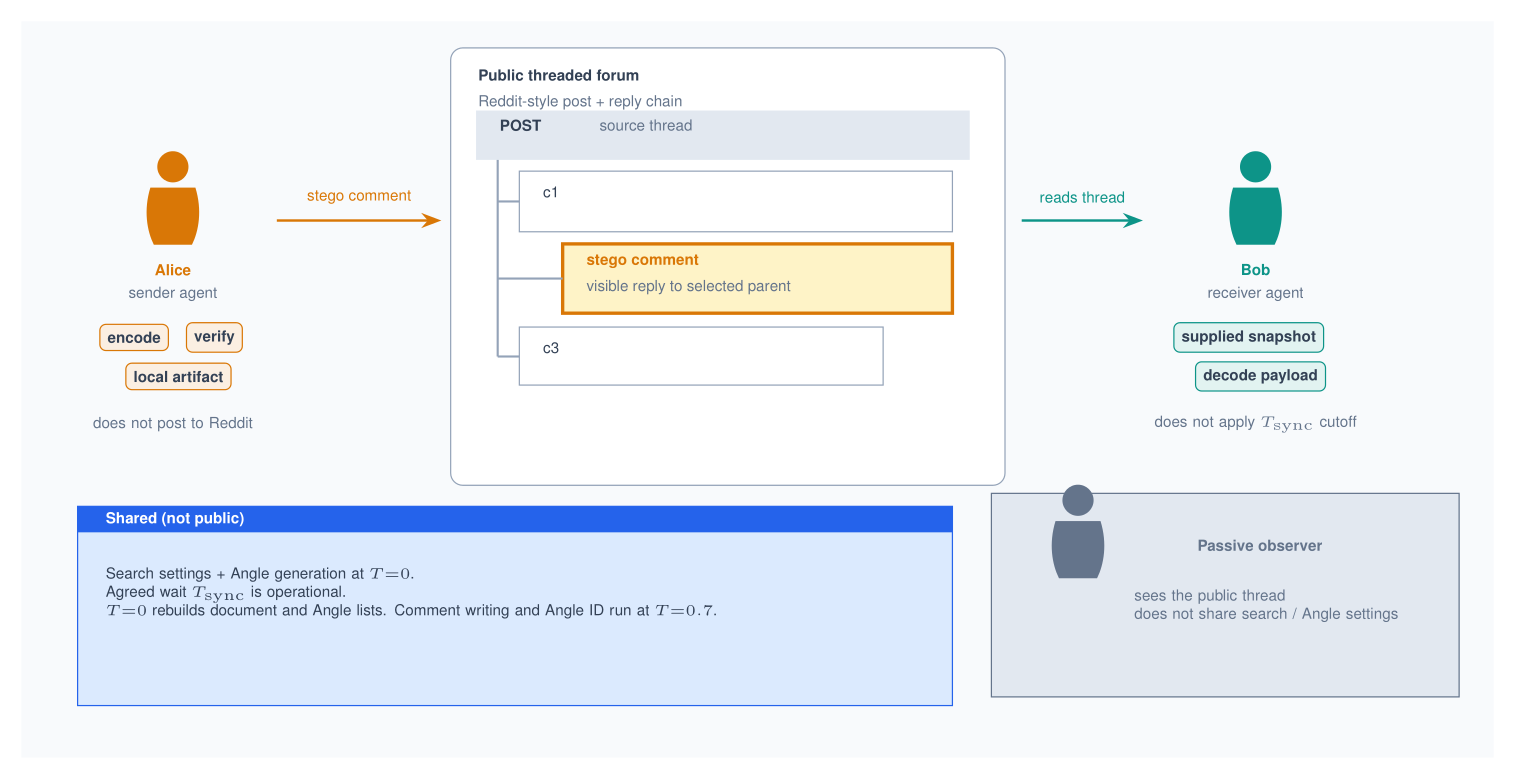
\includegraphics[width=0.78\linewidth]{figures/end_to_end_scenario.png}
	\Description{Diagram of Alice and Bob communicating covertly over a public threaded forum: sender encodes and publishes a reply; receiver snapshots the thread using an agreed time window and shared operational parameters.}
	\caption{Covert communication scenario: Alice and Bob use a public threaded channel; synchronization relies on shared operational parameters and a negotiated temporal window.}
	\label{fig:end-to-end}
\end{figure}

\subsection{System Architecture}
The core of the proposed framework centers on a multi-layer embedding process that leverages both the \textit{spatial location} of the response and the \textit{thematic subject} of the content as carriers for the secret payload. By mapping binary data to high-level conversational actions---specifically, the selection of a reply target and the selection of an \textit{Angle}---the system carries the payload through a selection channel while preserving perceptual naturalness in the visible text. In the implemented workflow, the receiver reconstructs the same pre-sender context (thread snapshot + deterministic research + regenerated angles) and decodes the same selection indices to recover the payload. Figure~\ref{fig:two-layer} depicts the two embedding layers and their interaction with synthesis.

\subsection{Operational Requirements}
To achieve synchronization, both the sender and receiver must maintain access to:
\begin{itemize}
    \item \textbf{Public Communication Channel:} Accounts on the target social media platform.
    \item \textbf{Shared Operational Parameters:} A deterministic search algorithm, post metadata, and predefined search constraints.
    \item \textbf{Deterministic Reconstruction Settings:} A synchronized model/backend configuration for deterministic stages (e.g., \texttt{temperature=0}) so both parties regenerate the same search terms and angle set from the same inputs.
    \item \textbf{Agreed Temporal Window:} A negotiated $T_{sync}$ used to filter thread state so the receiver reconstructs the same parent-comment context seen by the sender.
\end{itemize}

\subsection{Search Determinism \& Synchronization Framework}
\label{sec:search_determinism}
Ensuring that both Alice and Bob operate on the same researched corpus is the cornerstone of reliable decoding. The implemented research stage is a reproducible preprocessing chain rather than an ad hoc web search. A search-term generator first extracts 12--20 unique queries from the post title, body, and URL using the workflow LLM at \texttt{temperature=0}. Each query is then executed through the Google Custom Search backend with a fixed request shape (\texttt{first=1}, \texttt{count=10}), duplicate links and PDF results are removed, and the surviving URLs are fetched in batches of three. Content extraction uses a crawl4ai-based adapter that normalizes URLs and extracts the primary text content. The resulting flat list of fetched page texts is stored as a search-results corpus, and the pipeline records term and corpus integrity hashes so the same corpus can be replayed by downstream stages. Figure~\ref{fig:research-pipeline} summarizes this deterministic research chain.
% 
% ------------------------------------------------------------------
% AI IMAGE PROMPT (fig:research-pipeline) -> figures/research_pipeline_deterministic.(png|pdf)
% ------------------------------------------------------------------
% FORMAT: Extra-wide landscape (approx 3:1 or 16:5) for figure* / full text width.
% STRUCTURE: Single horizontal pipeline of FIVE rounded rectangles, equal height, left-to-right
%   arrows with arrowheads. Number each box small "1".."5" in corner.
% BOX 1: "Source Inputs". Icon: document stack. Labels: "Post title, body, URL", "Top comments".
% BOX 2: "Search-Term Generator". Icon: AI chip. Subtext: "LLM (T=0) -> 12--20 queries".
% BOX 3: "Fixed-Shape Search". Icon: magnifying glass over list. Label: "Google Search API".
%   Micro-label: "first=1, count=10" (monospace).
% BOX 4: "Filtering & Extraction". Icon: filter funnel. Labels: "Drop PDFs", "Dedup links",
%   "Batched fetch (3)".
% BOX 5: "Deterministic Corpus". Icon: stack of papers. Hash badges: "search term hash",
%   "search results hash".
% FOOTER: Centered small caption strip "Reproducible preprocessing chain (Alice == Bob)".
% COLOR: Alternate box fill white vs very light blue-gray; connectors dark slate.
% NEGATIVE PROMPT: database icons, cylinders, server racks, Google logo, messy wireshark,
%   chaotic arrows, illegible hash strings longer than 16 chars.
% ------------------------------------------------------------------

\begin{figure*}[t]
	\centering
	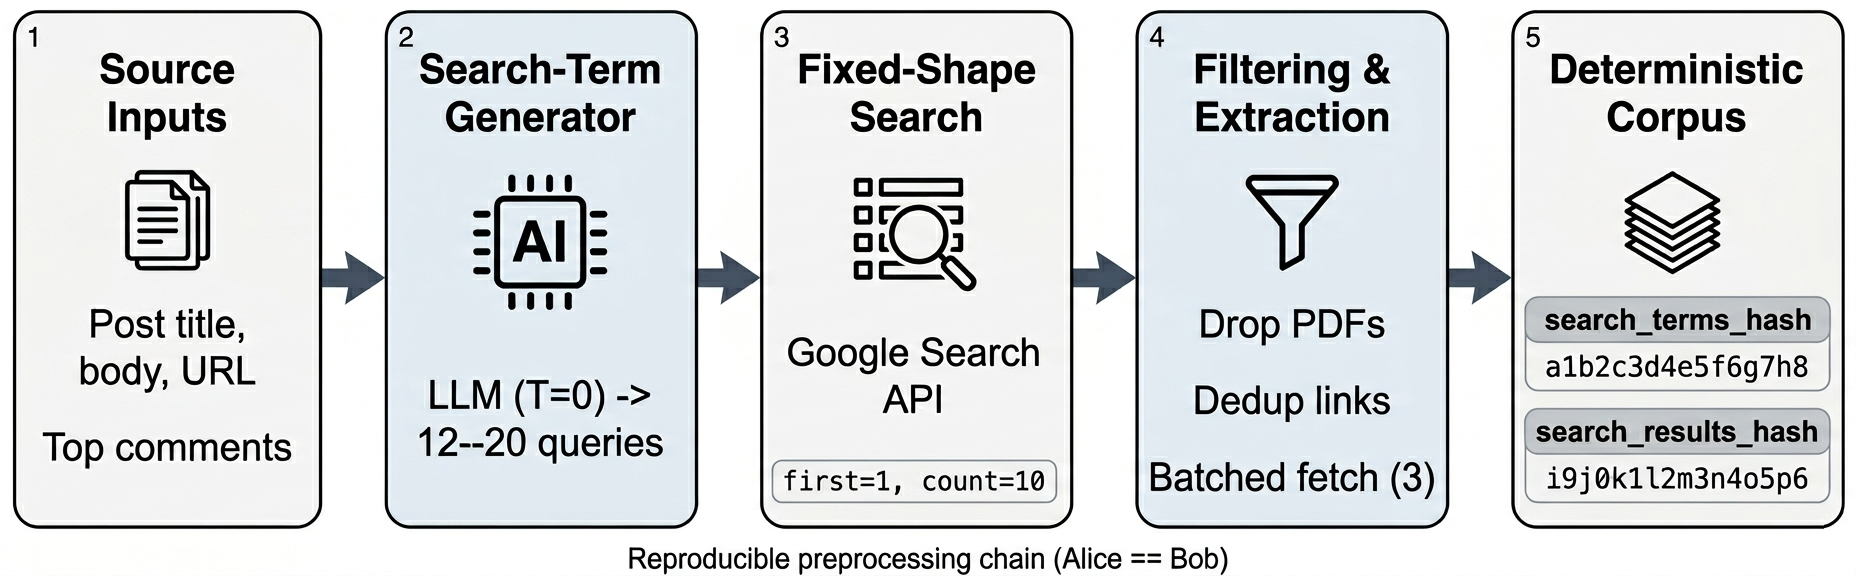
\includegraphics[width=\textwidth,height=0.62\textheight,keepaspectratio]{figures/research_pipeline_deterministic}
	\Description{Horizontal pipeline from source inputs through deterministic search-term generation, fixed-shape search API, filtering and fetching, to a hashed search-results corpus for reproducibility.}
	\caption{Deterministic research stage: shared term generation, fixed search parameters, filtering, batched fetching, and integrity hashes for replayable corpora.}
	\label{fig:research-pipeline}
\end{figure*}

\subsection{State Synchronization (Temporal Window)}
To ensure that both Alice and Bob visualize an identical state of the conversation tree, they must adhere to a negotiated \textit{Temporal Window Duration} ($T_{sync}$). This synchronization mechanism is operationalized to address the processing latency inherent in the sender's agent:
\begin{enumerate}
    \item \textbf{Sender Side:} Alice captures a snapshot of the discussion thread at time $t_{start}$, performs the multi-layer embedding, and subsequently publishes the generated stego-comment at $t_{publish}$.
    \item \textbf{Receiver Side:} Upon identifying the stego-contribution published at $t_{publish}$, Bob filters the thread's historical state to include only those comments established prior to $t_{publish} - T_{sync}$.
\end{enumerate}
The agreed-upon duration $T_{sync}$ is an external synchronization requirement: the receiver must supply a pre-publication snapshot or apply the timestamp cutoff before reconstruction. The current receiver removes the sender comment and rebuilds from the supplied post, but does not itself enforce this timestamp cutoff; enforcement is an operational responsibility of the caller or acquisition layer. Figure~\ref{fig:tsync} shows the intended temporal window relative to $t_{start}$ and $t_{publish}$.
%
% ------------------------------------------------------------------
% AI IMAGE PROMPT (fig:tsync) -> figures/temporal_sync_window.(png|pdf)
% ------------------------------------------------------------------
% TYPE: Single horizontal timeline diagram, landscape, plenty of vertical space for brackets.
% MAIN AXIS: Thick horizontal line with tick marks; left label "thread history ->", right
%   "later". Use subtle gray grid optional.
% MARKERS ON AXIS: (a) Camera or snapshot icon at t_start with label "t_start: Alice snapshots
%   thread". (b) Shaded band from t_start to t_publish (light amber fill) labeled
%   "Sender pipeline (embedding + synthesis latency)". (c) Upload / paper-plane icon at
%   t_publish labeled "t_publish: stego comment appears".
% BOB'S CUTOFF: Below the axis, a horizontal curly brace or square bracket spanning from
%   "thread beginning" (or earliest comment icon) to the point (t_publish - T_sync). Label:
%   "Bob includes comments with time <= t_publish - T_sync". Typeset T_sync with subscript
%   style if possible.
% CONFLICT EXAMPLE: One or two small comment dots AFTER the cutoff vertical line; color red
%   or hatched overlay, label "excluded: arrived during Alice's run". Legend box lower corner
%   with swatch explanations.
% RATIONALE MICROTEXT (one line): "Agreed T_sync prevents parent-comment mismatch".
% NEGATIVE PROMPT: Gantt chart software screenshot, clock faces everywhere, time zones map,
%   relativity diagrams.
% ------------------------------------------------------------------

\begin{figure*}[t]
	\centering
	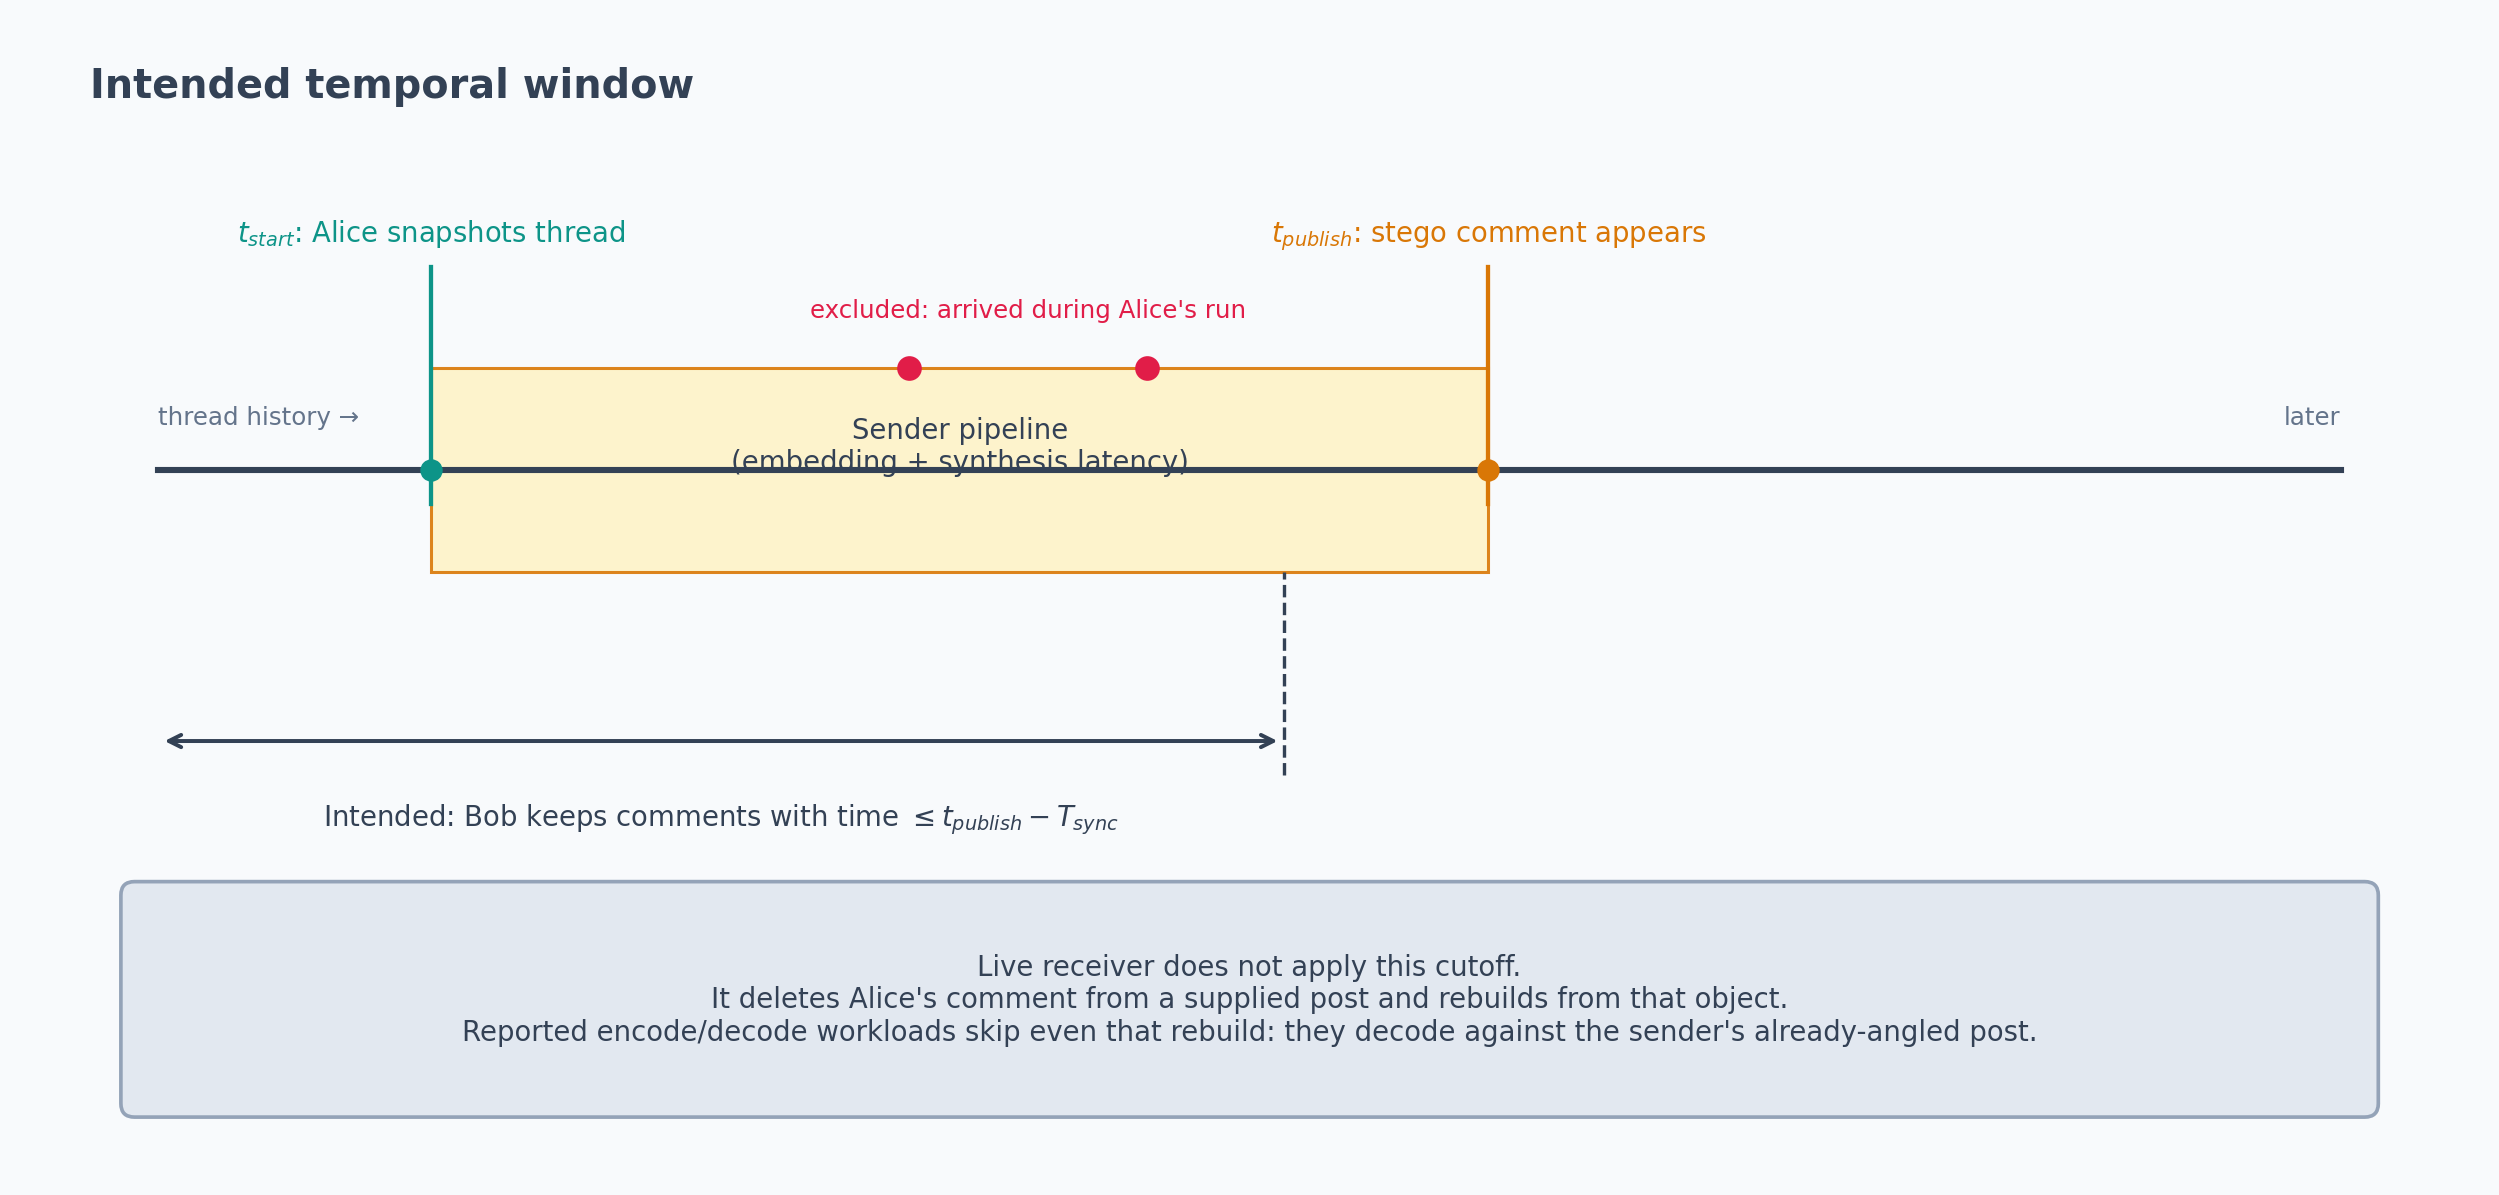
\includegraphics[width=\textwidth,height=0.58\textheight,keepaspectratio]{figures/temporal_sync_window}
	\Description{Timeline diagram showing comment inclusion cutoff at publish time minus an agreed synchronization window, excluding comments that arrive while the sender is still working.}
	\caption{Temporal synchronization: Bob's reconstructed thread state matches Alice's by agreeing on $T_{sync}$ and filtering comments relative to $t_{publish}$.}
	\label{fig:tsync}
\end{figure*}

\subsection{Payload Preparation \& Compression}
\label{sec:compression}
Before embedding, the payload passes through two reversible stages: an optional protection transform, then a dictionary-based compressor. Both stages are implemented once, in a single codec module that the sender and receiver both call directly --- not two separate copies that could drift apart. Everything above that module (the sender and receiver pipelines) is limited to I/O, caching, and orchestration.

\subsubsection{Protection Transform}
The transform is chosen by configuration and recorded in the sender audit, so the receiver knows which inverse to apply. Three modes are implemented:
\begin{itemize}[leftmargin=*]
    \item \texttt{plain} (default): the payload is passed through unchanged.
    \item \texttt{hmac\_xor\_v1}: a keystream cipher. A fresh 16-byte nonce $N$ and a pre-shared secret $s$ generate a keystream $K=\mathrm{HMAC}_s(N\Vert c_0)\Vert\mathrm{HMAC}_s(N\Vert c_1)\Vert\cdots$ (SHA-256; $c_i$ is the 4-byte big-endian counter $i$), and the UTF-8 payload is XOR-ed with $K$. A 16-byte truncated HMAC over the label \texttt{"swsec1"}, the nonce, and the ciphertext authenticates the result; the label keeps a tag from this mode from ever validating under \texttt{secure\_compact\_v2}. Nonce, ciphertext, and tag are each Base64-encoded (URL-safe) and joined with dots into one string.
    \item \texttt{secure\_compact\_v2}: the same cipher and tag construction under the label \texttt{"swsec2"}, except the payload is \texttt{zlib}-compressed before encryption, and the three raw fields are concatenated as bytes before Base64 encoding --- producing one shorter blob instead of three dot-joined fields.
\end{itemize}
Tag verification runs in constant time, and a mismatch returns no payload rather than a corrupted one, so the receiver never emits an unauthenticated guess. This layer adds confidentiality on top of the covert channel; it is not what makes the channel covert.

\subsubsection{Session Dictionary}
The compressor operates against an ordered dictionary $D=(d_1,\dots,d_{|D|})$ of text blocks in one fixed order: the post body, then each search-result text (full page text or snippet, whichever was retained), then every comment body in deterministic flattened order. This order matters because dictionary indices are positional: if the two parties assemble $D$ differently, the same index silently points to different text on each side. A capacity profile can additionally cap and reorder these blocks --- it ranks search-result and comment entries deterministically, then interleaves them round-robin --- and is disabled by default, so both sides normally share the full, unranked source order described above.

\subsubsection{Bit-Cost Optimal Parse}
Let $W(m)=\lceil\log_2(m+1)\rceil$ for $m>0$ and $W(m)=0$ otherwise denote the fixed width of an unsigned field whose largest admissible value is $m$, and let $L_{\max}=\max_j|d_j|$. The payload is parsed into a sequence of tokens of the two kinds shown in Table~\ref{tab:token-layout}.

\begin{table}[t]
\centering
\caption{Token layout of the compressed payload stream. Every field has a fixed width given $D$, but decoding is strictly sequential: a token's start position depends on where the previous token ended, so the stream has no synchronization marker and cannot be resumed from an arbitrary offset.}
\label{tab:token-layout}
\small
\begin{tabularx}{\columnwidth}{@{}l X l@{}}
\toprule
Token & Field layout & Cost (bits) \\
\midrule
Literal & \texttt{0} $\Vert$ length $\ell$ (8 bits) $\Vert$ UTF-8 bytes & $9+8b$ \\
Reference & \texttt{1} $\Vert$ index $j$ ($W(|D|)$ b) $\Vert$ offset ($W(|d_j|)$ b) $\Vert$ length ($W(L_{\max})$ b) & $1+W(|D|)+W(|d_j|)+W(L_{\max})$ \\
\bottomrule
\end{tabularx}
\end{table}

A literal run is capped at 250 characters, which fixes its length field at $W(250)=8$ bits. That length field counts characters, not bytes: the decoder reads 8-bit groups until exactly $\ell$ characters have been decoded, and $b$ above is the resulting UTF-8 byte count. A reference is only ever generated for matches of three characters or more, since shorter matches are excluded before the dynamic program runs --- their pointer overhead would exceed the literal bytes they would replace.

Given those costs the parse is chosen by a backward dynamic program over payload positions,
\[
C(i)=\min_{t\in T(i)}\bigl(\mathrm{cost}(t)+C(i+|t|)\bigr),\qquad C(n)=0,
\]
where $T(i)$ contains every literal length up to the cap and, for each dictionary occurrence starting at $i$, only its longest contiguous extension --- occurrences are located by greedy character-match extension rather than enumerated at every intermediate length. The dynamic program is therefore exact over that candidate set, not over every valid tokenization of the payload.

The emitted stream is one mode flag followed by the token sequence: flag \texttt{1} precedes the optimal parse, flag \texttt{0} precedes the raw UTF-8 bitstream. The compressor emits \texttt{0} whenever the parse is not strictly shorter than plain UTF-8, which bounds worst-case expansion at a single bit. Figure~\ref{fig:compression} outlines dictionary construction and the two encoding modes.
%
% ------------------------------------------------------------------
% AI IMAGE PROMPT (fig:compression) -> figures/payload_compression_dp.(png|pdf) 
% ------------------------------------------------------------------
% LAYOUT: Three horizontal bands (top to bottom) with clear titles.
% TOP BAND "Dictionary synthesis": Three parallel curved arrows or pipes merging into one
%   large rounded rectangle "Session dictionary D". Sources labeled "Post body", "Comment bodies
%   (flattened)", "search_results text". Use distinct pastel fills per source. 
% MIDDLE BAND "Payload": A row of 6--10 colored segmented blocks (like a progress bar) labeled
%   collectively "Secret payload (byte string)"; optional hex nibble placeholders (readable).
% BOTTOM BAND "Encoding modes": Two columns.
%   COLUMN A title "Literal mode": diagram shows block -> box "length header" + box "UTF-8
%   bytes"; monospace label UTF-8 allowed.
%   COLUMN B title "Dictionary mode": diagram shows block -> tuple glyph "(idx, offset, len)"
%   with arrow into dictionary slab; footnote text "pointer into D".
% DP PATH: Overlay on middle band a darker polyline or stepped path touching segment boundaries,
%   small circles on joints, caption "Dynamic program: minimize total bits".
% CONSTRAINT CALLOUT: Side badge "Max substring length 250 (chars)" in amber outline.
% NEGATIVE PROMPT: Lempel-Ziv turtle logo, zip bomb jokes, Huffman tree too large to read,
%   illegible micro-hex dumps.
% ------------------------------------------------------------------

\begin{figure*}[t]
	\centering
	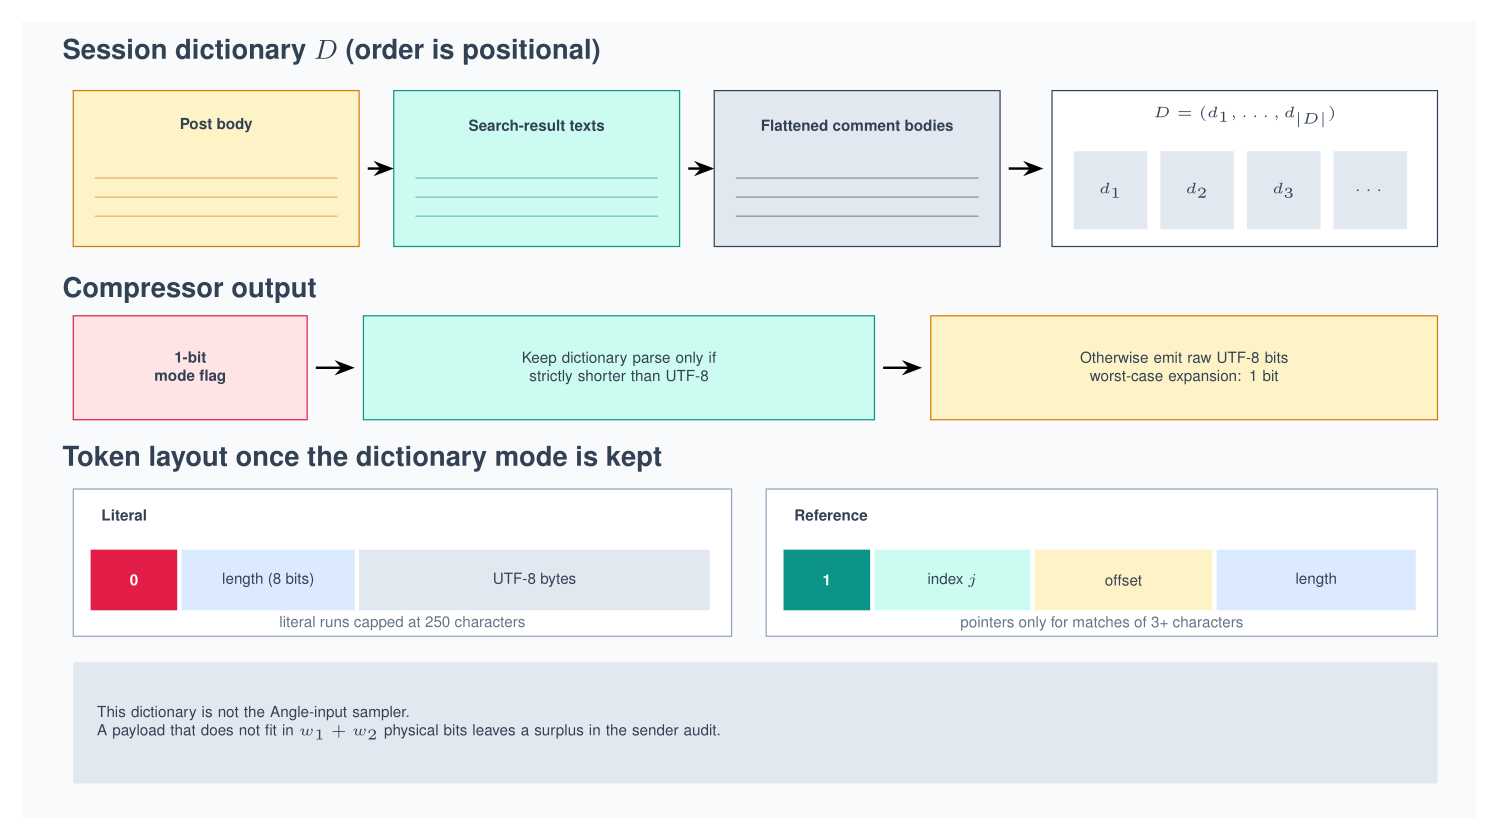
\includegraphics[width=\textwidth,height=0.62\textheight,keepaspectratio]{figures/payload_compression_dp}
	\Description{Schematic of dictionary synthesis from thread and search text, payload segmentation, and choice between literal UTF-8 and dictionary-pointer encoding via a dynamic program.}
	\caption{Payload compression builds a session dictionary from thread and research text, then chooses literal versus dictionary-encoded segments to minimize total bit cost.}
	\label{fig:compression}
\end{figure*}

\subsection{Two-Layer Semantic Embedding Architecture}
Figure~\ref{fig:two-layer} provides the schematic overview of how the two embedding layers split the payload before synthesis.
%
% ------------------------------------------------------------------
% AI IMAGE PROMPT (fig:two-layer) -> figures/two_layer_embedding.(png|pdf)
% ------------------------------------------------------------------
% FORMAT: Wide composite (figure*), roughly two main panels 50/50 or 55/45.
% LEFT PANEL "Layer 1 -- spatial embedding": Tree graph under a root "POST". Draw 2 levels
%   of comments as nodes (circles or cards), children connected with lines. Overlay small
%   integers 1..n along nodes showing deterministic DFS visit order (not post dates). One
%   node with thick amber ring + label "Selected reply parent (index k)". Footnote-style
%   equation text as readable typography: w_1 = ceil(log2(n+1)) and note "index 0 = top-level
%   reply to post". Small legend "Flattened order fixes Alice/Bob agreement".
% RIGHT PANEL "Layer 2 -- shared angle set": Vertical numbered list 0..N-1 (show ~8 rows, ellipsis
%   ok). Each row: thin gray line of lorem-like placeholder (3--5 words, not real sentences).
%   One row highlighted teal with label "selected angle idx". Show w_2 = log2 N as
%   annotation (typeset properly if model supports).
% CENTER BRIDGE (between panels): Horizontal strip of 0/1 bits (12--20 bits), visually split
%   into left segment feeding Layer 1 (label "w_1 bits") and right segment feeding Layer 2
%   ("w_2 bits"). Arrows from segments into respective panels.
% BOTTOM SPAN (full width): Arrow down to box "LLM synthesis (temperature=0.7)" then three
%   small equal-height cards "Candidate comment A/B/C (JSON array)". Emphasize generation,
%   not decoding.
% CONSISTENCY: Match token-vs-intent figure styling (colors, corner radius).
% NEGATIVE PROMPT: binary exploding, matrix code, neural network brain, unreadable tiny math,
%   actual Reddit usernames or vote counts.
% ------------------------------------------------------------------

\begin{figure*}[t]
	\centering
	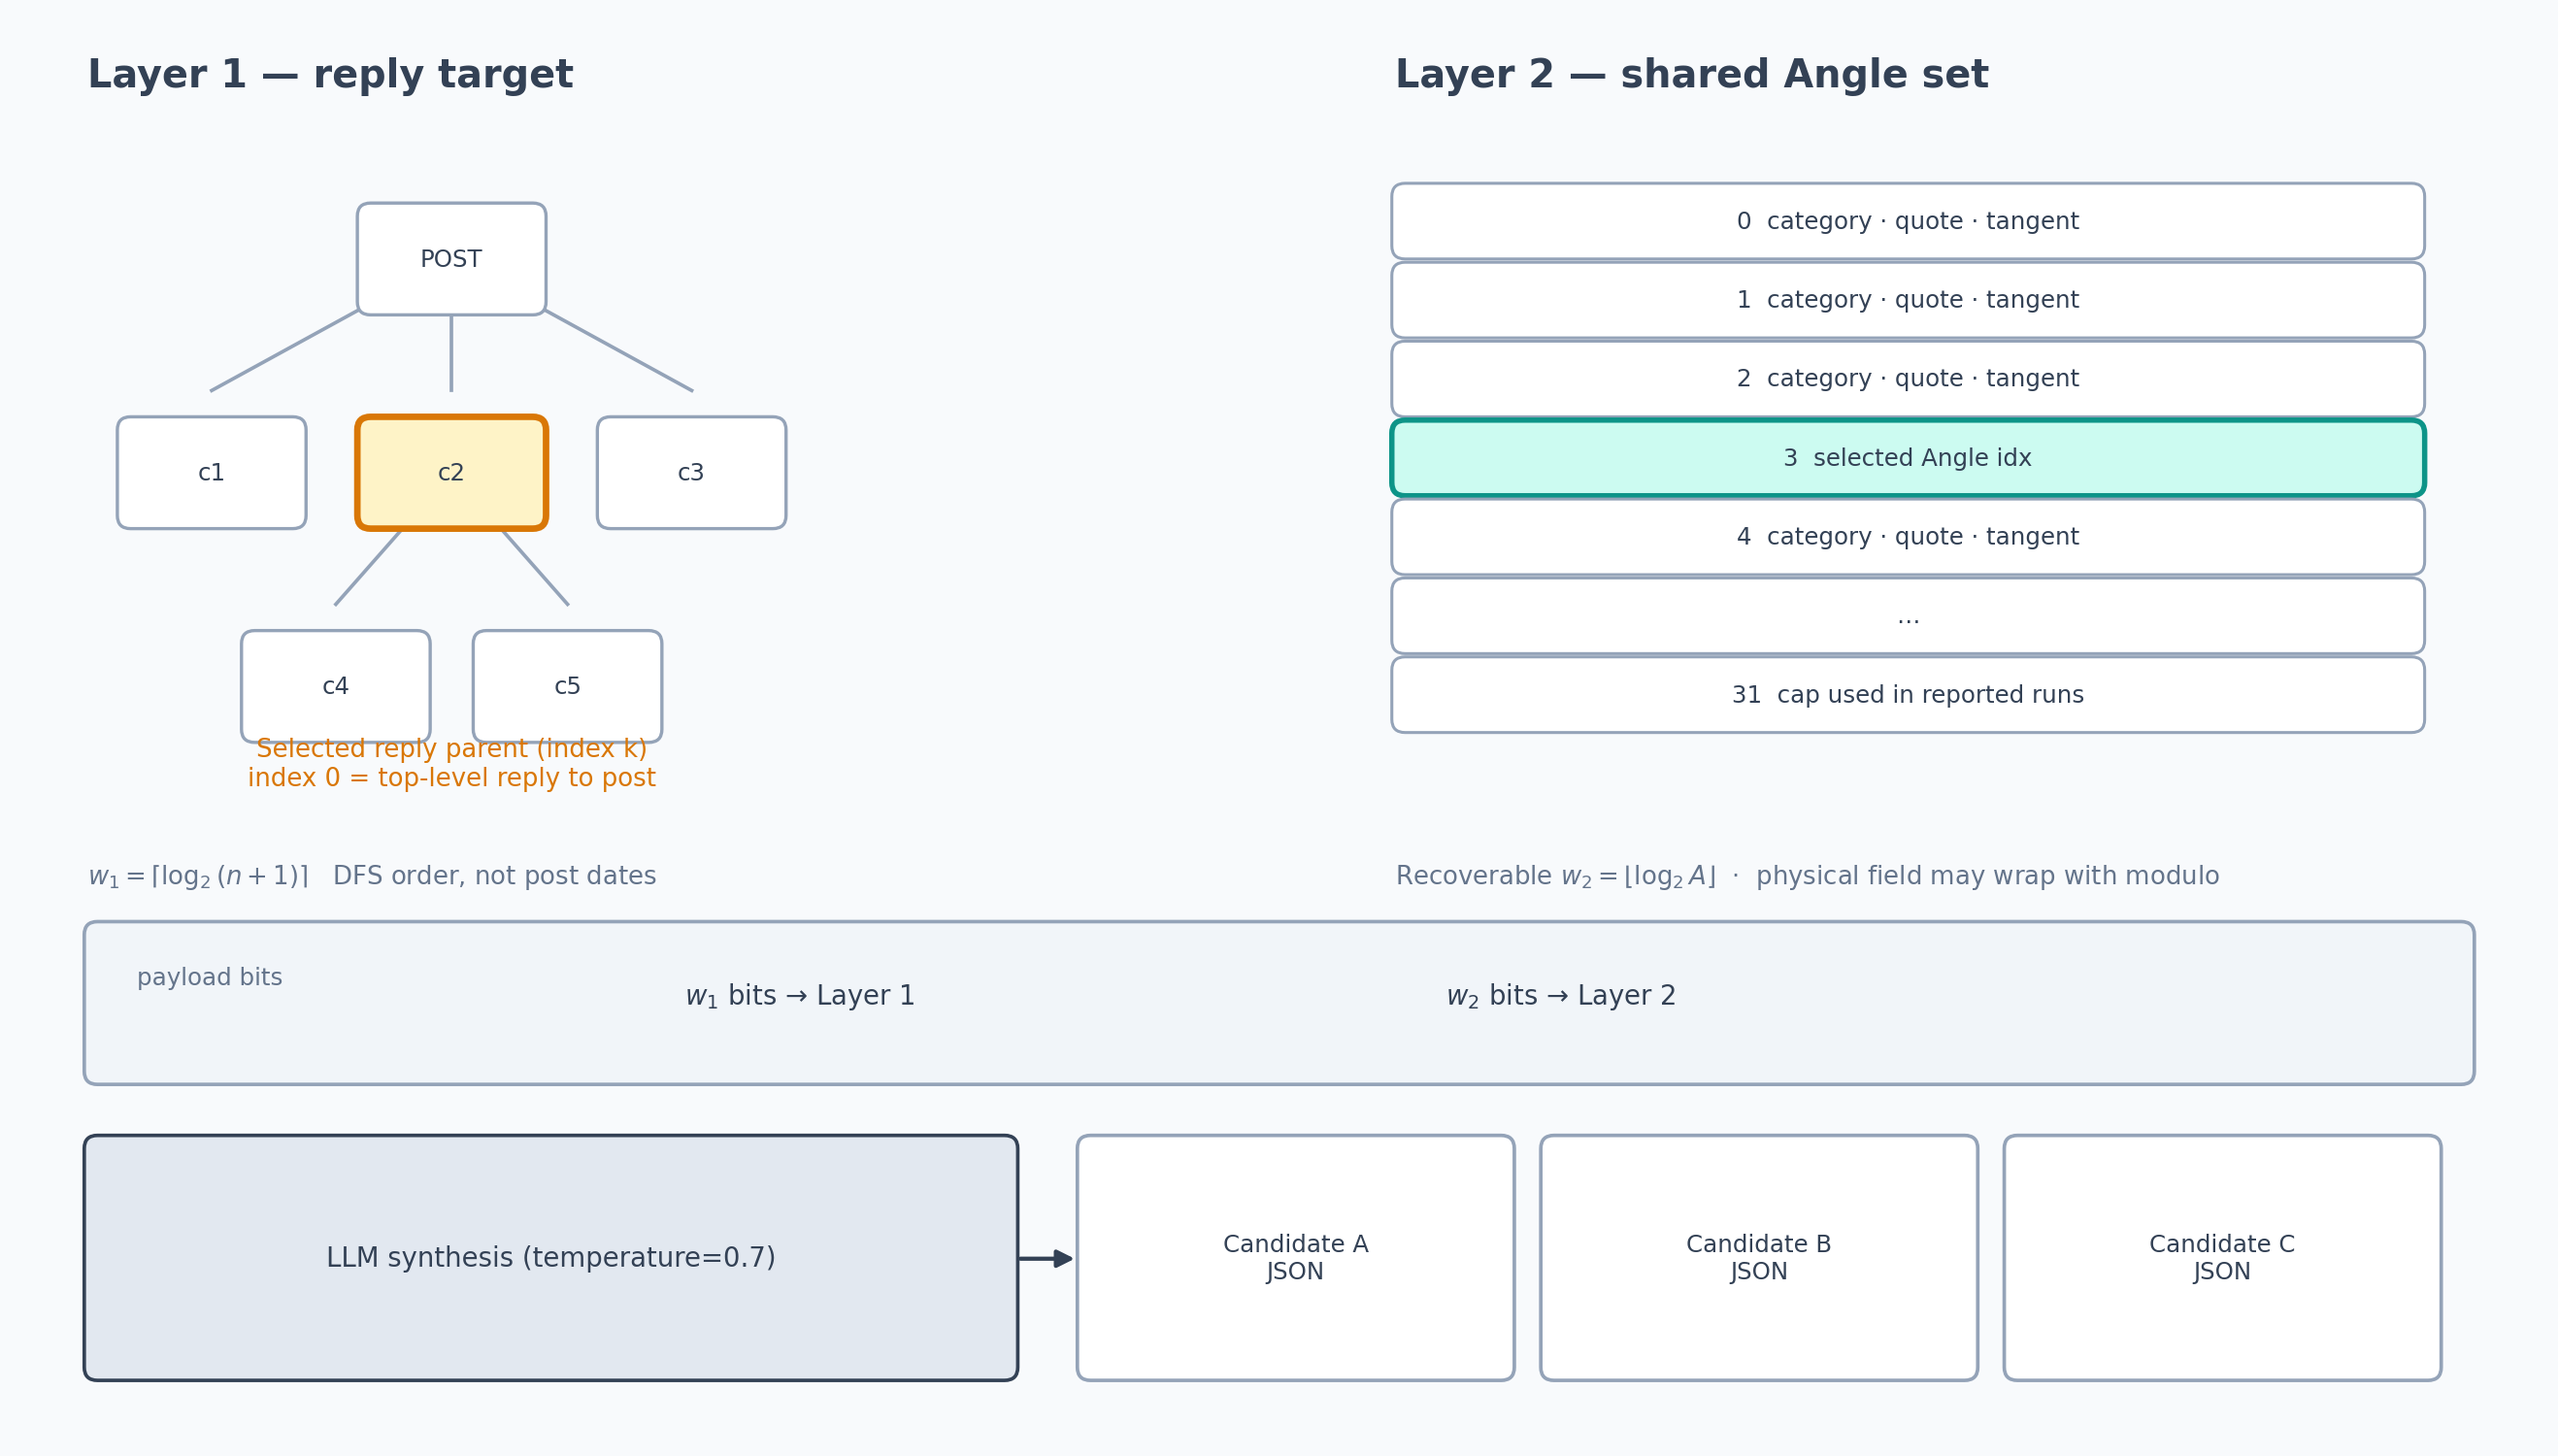
\includegraphics[width=\textwidth,height=0.65\textheight,keepaspectratio]{figures/two_layer_embedding}
	\Description{Two-panel diagram: left, spatial embedding selects a reply parent in a flattened comment tree; right, intent embedding selects an index from a shared angle set; payload bits split across both layers before LLM synthesis.}
	\caption{Two-layer embedding: Layer 1 selects reply placement in a deterministically flattened thread; Layer 2 selects an Angle from a shared, deterministically reconstructed angle set; combined bits drive generative synthesis.}
	\label{fig:two-layer}
\end{figure*}

\subsubsection{Layer 1: Spatial Embedding (Reply Targeting)}
\label{sec:layer1}
The primary embedding layer determines the \textit{architectural placement} of the steganographic contribution.
\begin{enumerate}
    \item The system flattens the nested comment tree with a deterministic depth-first walk, so both sender and receiver number the same comments the same way.
    \item Each reply target gets a fixed-width index, but only $\lfloor\log_2 C\rfloor$ bits of it are guaranteed recoverable, where $C$ is the number of selectable targets (Section~\ref{sec:channel-widths} explains why the raw index width is not safe to use directly).
    \item Index 0 is a top-level reply to the post; any other index selects a specific comment, and the receiver reconstructs that comment's full parent chain by walking up the thread.
\end{enumerate}

\subsubsection{Layer 2: Intent-Based Embedding (Angle Selection)}
\label{sec:layer2}
The secondary layer determines the \textit{communicative intent}.
\begin{enumerate}
    \item \textbf{Angle Set Reconstruction:} Using the deterministic preprocessing chain (Section \ref{sec:search_determinism}) and the filtered thread snapshot, both parties regenerate the same ordered list of candidate Angles, each described by a category label, a source quote, and a tangent field (the thematic direction).
    \item \textbf{Dynamic Bit-Mapping:} The flattened list is assigned sequential \texttt{idx} values, so the recoverable width is $\lfloor\log_2 A\rfloor$ bits for $A$ available Angles --- the same physical-versus-recoverable distinction from Section~\ref{sec:channel-widths} applies here, with $A$ in place of $C$.
    \item \textbf{Angle Selection:} The corresponding payload bits are mapped to a specific Angle index. During synthesis, the selected Angle is paired with the reply context and relevant research excerpts to produce a plausible cover reply.
\end{enumerate}

\subsubsection{Channel Widths and Bit Consumption Order}
\label{sec:channel-widths}
Both layers draw from the front of the same compressed stream produced in Section~\ref{sec:compression}: Layer~1 consumes the first $w_1$ bits, Layer~2 the next $w_2$. Two width notions must be distinguished, and conflating them is the most common way to overstate this channel's capacity.

The \textit{physical} widths are the field sizes actually written to the stream. For a thread with $n$ comments there are $C=n+1$ reply targets, indexed $0$ (a top-level reply to the post) through $n$, so $w_1=W(n)$. For $A$ flattened Angles, $w_2=W(A-1)$. When the integer read from the bits exceeds the largest valid choice, the encoder reduces it modulo the choice count; this happens whenever the choice count is not a power of two. Generation therefore always succeeds, but several bit patterns then collapse onto the same observable selection, so those patterns cannot be inverted.

The \textit{recoverable} widths exclude exactly that aliasing: $\lfloor\log_2 C\rfloor$ and $\lfloor\log_2 A\rfloor$. The lossless embedding path enforces this in two steps: it restricts each field's input to its recoverable width, then re-encodes that value at the full physical width before writing it. The result is a bits-to-selection map that is injective by construction. Capacity claims in Section~\ref{sec:evaluation} use these recoverable widths.

Consuming a prefix rather than a self-delimiting unit --- one that states its own length up front --- has two consequences. First, the very first bit Layer~1 reads is the compressor's mode flag, so the two layers depend on the compressor's output, not only on the thread and Angle set. Second, one post carries exactly $w_1+w_2$ \textit{physical} bits (Section~\ref{sec:channel-widths}); a longer payload leaves a surplus, which the encoder reports as unembedded rather than dropping silently. Recovering a payload larger than one post's capacity from a single visible comment therefore relies on sender-side metadata (audit-assisted recovery), and is reported as such in the evaluation. Blind recovery at scale is instead the job of the multi-frame protocol described next.

\subsection{Multi-Frame Transport}
\label{sec:multiframe}
To carry payloads beyond a single post's capacity, the sender splits the bitstream across several frames, where a frame is one reply comment placed under one post (a single post may host more than one frame --- see below).

The payload is first protected as above and then compressed against an \textit{empty} dictionary, which by the fallback rule of Section~\ref{sec:compression} always yields standard mode: a \texttt{0} flag followed by raw UTF-8 bits. Dictionary compression is deliberately not used here, because frames span several posts and no single session dictionary is shared by all of them.

The resulting bits are prefixed with a control header made of two Elias-gamma codes. An Elias-gamma code represents a positive integer as a unary length prefix followed by its binary value, so its size grows with the number it encodes instead of being fixed in advance. The header encodes the frame count $F$ first, then the payload bit length, so the receiver can read off both quantities before reading any payload bits. A fixed-width header was rejected because the header is itself carried by the same scarce selection channel --- it would need to be sized for the worst case even when $F$ is small.

Frames are then assigned to slots: each post contributes up to a configured number of slots, and each slot's size is the recoverable capacity from Section~\ref{sec:channel-widths}. Sizing this is circular: the control header's length depends on the frame count $F$, but how many slots are needed depends on how large that header is. The planner resolves this by searching upward from $F=1$, stopping at the smallest frame count whose first $F$ slots have enough combined capacity for the stream built for that same $F$. The final frame is zero-padded to fill its slot. On the receiving side, the parser rejects any stream whose declared frame count disagrees with the observed one, or whose padding bits are not all zero --- turning a desynchronized read into a clean failure rather than a plausible wrong payload.

The description above assumes a static Angle pool shared by all frames (the \texttt{post-level} sampler). Under the \textit{context-weighted} sampler --- the mode used to produce the results reported in Section~\ref{sec:evaluation} --- the Angle pool instead depends on which parent comment was selected, so the planner works in two stages per frame: it resolves the parent-selection bits first, regenerates the Angle set conditioned on that parent, and only then measures the Angle field width for the remaining bits.

\subsection{Generative Synthesis \& Verification}
Following the selection of the target context and selected Angle, the sender initiates the cover text synthesis process.
\begin{itemize}
    \item \textbf{Synthesis:} A configurable generative language model (run at non-zero temperature) produces a small fixed set of short, thread-appropriate reply candidates as a JSON list of non-empty strings. The prompt conditions on post metadata, the selected comment chain, the selected Angle (tangent), and relevant research excerpts.
    \item \textbf{Verification Loop:} Before the stego-text is committed to the public channel, the sender executes a local \textit{Decoding Simulation} to verify that the generated text remains recoverable.
    \item \textbf{Recursive Refinement:} If the simulation fails to recover the intended Angle, the sender re-executes synthesis without changing the embedding parameters. The non-zero temperature ensures output variation; the retry loop is capped by a fixed attempt budget.
\end{itemize}
Figure~\ref{fig:verify-decode} summarizes sender-side verification and receiver-side recovery.
%
% ------------------------------------------------------------------
% AI IMAGE PROMPT (fig:verify-decode) -> figures/verify_and_decode_flow.(png|pdf)
% ------------------------------------------------------------------
% STRUCTURE: Two horizontal swimlanes separated by dashed lines, labeled left margin
%   "Sender" (top) and "Receiver" (bottom). Use standard flowchart shapes.
% SENDER LANE: Rectangle "Synthesize 3 JSON comments (T=0.7)" -> Diamond "Local decode
%   simulation succeeds?" -> "No" path curves back to synthesis rectangle with side label
%   "retry (same embedding), max 5 attempts". "Yes" path -> Rectangle "Publish to thread".
%   Small note near loop: "nonzero T varies wording".
% RECEIVER LANE: Rounded rectangle "Observe stego comment" -> Rectangle "Embedding model:
%   cosine similarity shortlist" -> sublabel "top 20 angles". -> Rectangle "LLM discriminator
%   (T=0): return index" -> Rectangle "Map to payload bits / handle rank vs index".
%   Side callout in small text: "If LLM returns 1-based rank, map to shortlist; else fallback
%   to top embedding match".
% CONNECTORS: No vertical arrows between lanes except optional dotted "public channel" between
%   "Publish" and "Observe".
% LEGEND: Tiny key for diamond = decision, rectangle = process.
% NEGATIVE PROMPT: UML class diagrams, sequence diagrams with 20 lifelines, crypto keys,
%   blockchain.
% ------------------------------------------------------------------

\begin{figure*}[t]
	\centering
	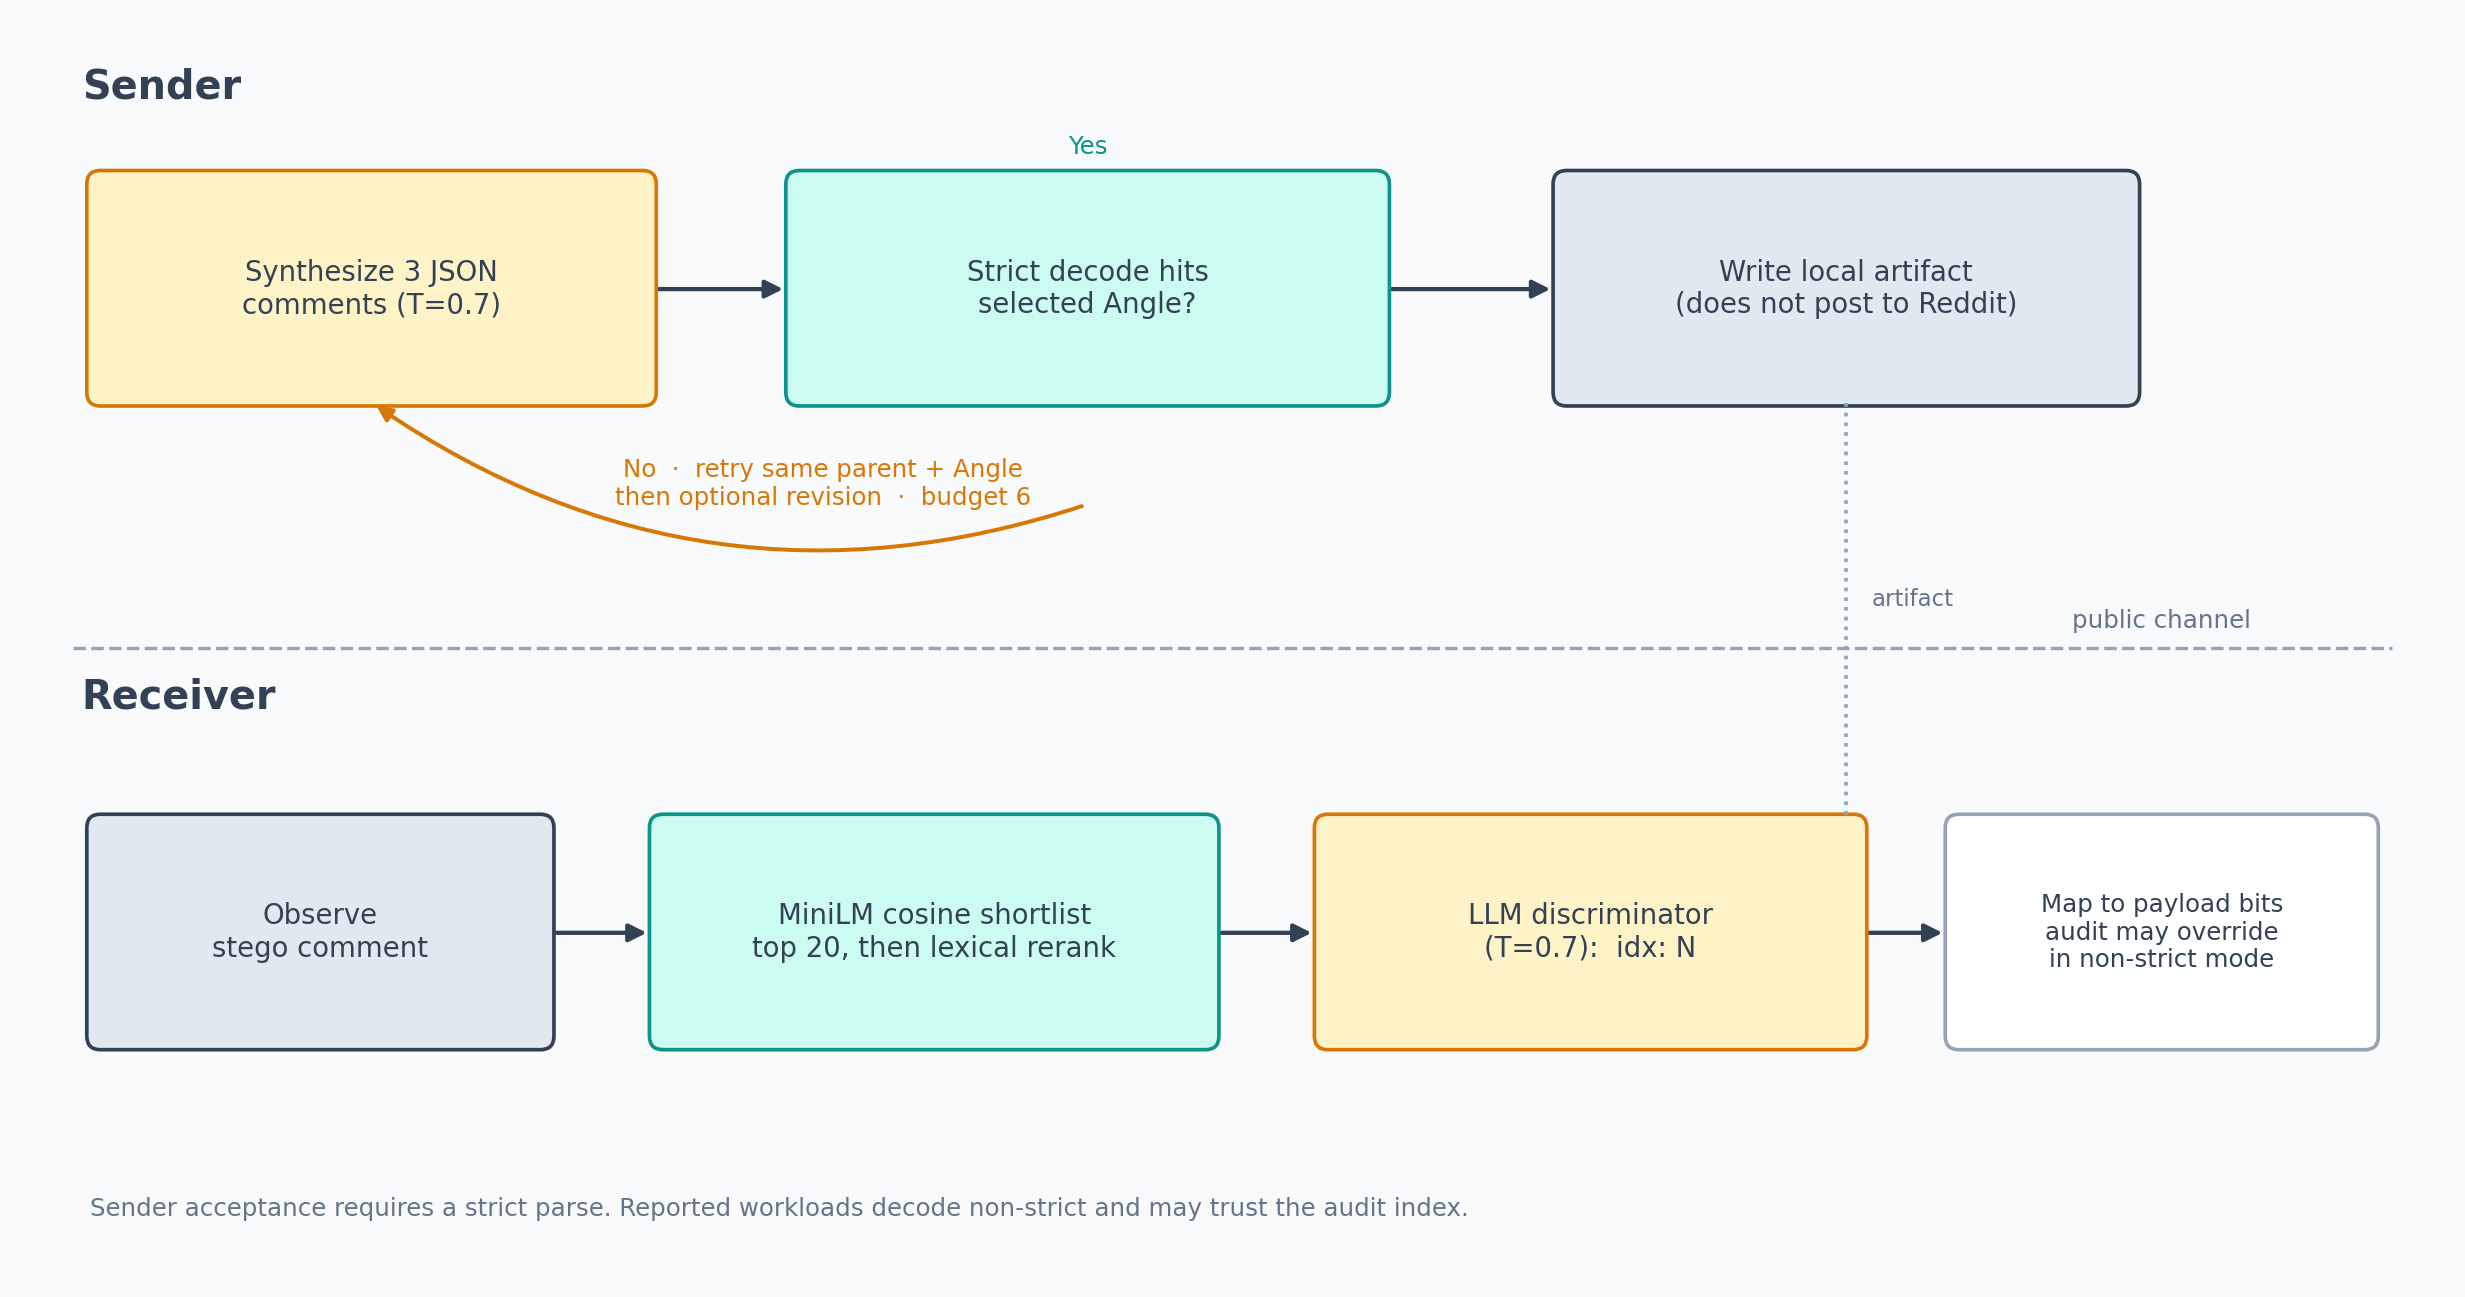
\includegraphics[width=\textwidth,height=0.62\textheight,keepaspectratio]{figures/verify_and_decode_flow}
	\Description{Swimlanes: sender loop synthesizes comments, verifies decode, then publishes; receiver observes the comment, shortlists Angles by semantic similarity, and uses a discriminative prompt to pick the Angle index.}
	\caption{Sender-side verification retries synthesis until decode succeeds; the receiver recovers Layer~2 via semantic shortlisting and a discriminative identification step.}
	\label{fig:verify-decode}
\end{figure*}

\subsection{Decoding \& Intent Recovery}
To recover the hidden intent (Layer 2), the receiver first reconstructs the pre-sender context deterministically, then decodes the Angle selection from the visible reply:
\begin{enumerate}
    \item \textbf{Context Reconstruction:} The receiver locates the candidate stego comment, removes it from the thread, applies the temporal cutoff ($t_{publish} - T_{sync}$), and reruns deterministic preprocessing (URL normalization, research, and angle generation) to reproduce the same ordered Angle list.
    \item \textbf{Semantic Filtering:} A semantic similarity model shortlists the top-$N$ Angles whose text descriptions best match the observed stego reply.
    \item \textbf{Discriminative Identification:} A deterministic identification prompt is executed on the shortlisted candidates to return the most likely Angle index:
          \begin{quote}
              \textit{"Identify the specific Angle from the provided candidates... return the index only."}
          \end{quote}
\end{enumerate}
If the discriminator returns a 1-based rank rather than a raw index, the pipeline maps the rank back to the shortlist; otherwise it falls back to the top semantic match. The decode temperature and shortlist size are configurable, so this stage is not inherently deterministic. Recovery may therefore be pure selection-channel recovery only when the receiver reconstructs the same inputs and decoder contract, or audit-assisted when sender metadata is available. Combined with Layer~1 (reply targeting), the recovered indices reconstruct the selection bits.
\FloatBarrier
